\documentclass{article}
\usepackage[utf8]{inputenc}

\title{Machine Learning, Sentence Trees}
\author{Bartłomiej Szymański}
\date{23 March-4 April 2019}

\usepackage{natbib}
\usepackage{graphicx}
\usepackage{hyperref}
\usepackage{float}

\begin{document}

\maketitle

\section{Tokenization of sentences, words}
The dataset that is being provided to us contains multiple sentences. NLTK library for Python allows to tokenize\cite{Tokenization} the text into individual sentences with any given delimiters, and then each of the sentences into actual words. The order of operation in this case is important, because it allows to create multidimensional arrays where each sentence would be represented by an array stored in an array of sentences.\\ \\
Consider a set of sentences like:
\begin{quote}
This thing seemed to overpower and astonish the little dark-brown dog, and wounded him to the heart. He sank down in despair at the child's feet. When the blow was repeated, together with an admonition in childish sentences, he turned over upon his back, and held his paws in a peculiar manner. At the same time with his ears and his eyes he offered a small prayer to the child.
\end{quote}
The desired form of this sentence after applying Sentence Tokenization and then Word Tokenization is:
\begin{verbatim}
[
['This', 'thing', 'seemed', 'to', 'overpower', 'and', 'astonish', 
'the', 'little', 'dark-brown', 'dog', ',', 'and', 'wounded', 
'him', 'to', 'the', 'heart', '.'],
['He', 'sank', 'down', 'in', 'despair', 'at', 'the', "child's", 
'feet', '.'],
['When', 'the', 'blow', 'was', 'repeated', ',', 'together', 
'with', 'an', 'admonition', 'in', 'childish', 'sentences', ',', 
'he', 'turned', 'over', 'upon', 'his', 'back', ',', 'and', 'held', 
'his', 'paws', 'in', 'a', 'peculiar', 'manner', '.'],
['At', 'the', 'same', 'time', 'with', 'his', 'ears', 'and', 'his', 
'eyes', 'he', 'offered', 'a', 'small', 'prayer', 'to', 'the', 
'child', '.']
]
\end{verbatim}
You can achieve this form by using the following code from the NLTK library (make note that as of version 3.3, a fragment of functionality became deprecated and might get removed before we finish the assignment, the code below is the up-to-date version of the issue)\cite{Demo of TweetTokenizer}\cite{New NLTK Tokenizer}:
\begin{verbatim}
    #the old version of NLTK
    from nltk.tokenize import TweetTokenizer, sent_tokenize
    tokenizer_words = TweetTokenizer()
    tokens_sentences = [tokenizer_words.tokenize(t) for t in 
    nltk.sent_tokenize(input_text)]
    print(tokens_sentences)
    
    #the new version of NLTK
    cd ~
    wget http://nlp.stanford.edu/software/
    stanford-corenlp-full-2018-02-27.zip
    
    unzip stanford-corenlp-full-2018-02-27.zip
    cd stanford-corenlp-full-2018-02-27
    java -mx4g -cp "*" edu.stanford.nlp.pipeline.StanfordCoreNLPServer \
    -preload tokenize,ssplit,pos,lemma,ner,parse,depparse \
    -status_port 9000 -port 9000 -timeout 15000 & 
    
    from nltk.parse import CoreNLPParser
    parser = CoreNLPParser(url='http://localhost:9000')
    list(parser.tokenize(sentence))
\end{verbatim}
To further optimize the list of sentences it is possible to remove punctuation from each of those sentences. Note that by this you might remove some context from the sentences that might become a useful feature in the feature space for Machine Learning.
\section{Exploring Sentence Trees}
To simplify this concept for the sake of our assignment, each sentence in any language can be deconstructed into a tree. To begin creating a Sentence Tree, it is necessary to assign PoS (Parts-of-Speech)\cite{POS} labels to every word in a given sentence.

\subsection{Simple PoS Trees}
In NLTK, this can be done using this code.
\begin{verbatim}
#old version
sentences = [nltk.pos_tag(sent) for sent in sentences]

#new version
pos_tagger = CoreNLPParser(url='http://localhost:9000', tagtype='pos')
list(pos_tagger.tag(sentence_array))
\end{verbatim}
Where sentences is an array of tokenized sentences, just like in the first section of this document. The output of this operation for a sentence
\begin{verbatim}
    The blogger taught the reader to chunk.
\end{verbatim}
becomes:
\begin{verbatim}
    [('The', 'DT'),
      ('blogger', 'NN'),
      ('taught', 'VBD'),
      ('the', 'DT'),
      ('reader', 'NN'),
      ('to', 'TO'),
      ('chunk', 'VB'),
      ('.', '.')]
\end{verbatim}
Description of all the labels NLTK can return is located here\cite{POS labels}. \\
In this case, the tree of this sentence looks like follows:
\begin{figure}[htb!]
    \centering
    
\includegraphics[width=\textwidth]{nickcdryanblog2.png}
    \caption{PoS labeled tree}
\end{figure}\\
This is a very basic tree. It does not give much information on dependencies between words, but is big enough to construct a basic feature space as long as you apply Chunking. Chunking is the process of grouping words together to provide us relevant blocks of information when it comes to sentences. \\ \\
The project that we've picked consists extracts PRP/PRP\$s from the sentences (personal pronouns, such as "He" or "his") and chunks of NNPs/NNPSs (Proper Nouns and Proper Nouns in Plural respectively, for example "Manchester United" or "Americans"). \\ \\
The easiest way to create chunks of NNPs and NNPSs is to connect cases when NNPs and NNPSs show up one after another, keeping in mind that punctuation does break the NNP blocks.
Consider the 158th entry of the dataset:
\begin{quote}
    On 17 June 2005, after 12 years at Birmingham, Bennett transferred to Leeds United who already had Scottish international goalkeeper Neil Sullivan as first-choice goalkeeper. Despite playing the pre-season friendlies, he was limited to four league appearances during the 2005-06 season, obtained deputising for the injured Sullivan.
\end{quote}
Though Birmingham and Benett are words that are next to one another, there is a comma between those two words, making them separate chunks of NNPs. Leeds United and Neil Sullivan will both be two-word long chunks of NNPs. \\ \\
The most simple feature space that can be extracted from this entry for this project would contain the following phrases:
\begin{verbatim}
    Birmingham
    Benett
    Leeds United
    Neil Sullivan
    he
    Sullivan
\end{verbatim}
Make note that while looking at this simple feature space, it might become tempting to pinpoint Neil Sullivan as the person to whom the pronoun is referring, the actual answer in this example is "Benett", not "Neil Sullivan". This is why this size of a feature space is \textbf{not} representative enough for the whole sentence.\\ \\

\subsection{Noun Phrases vs Verb Phrases}
The sentence can be subjected to the process of more advanced chunking, known as Shallow Parsing. By combining the labels of words together, it is possible to create your own context-free grammars that would form two types of chunks worth considering:
\begin{itemize}
    \item Noun Phrase (NP), a block that spans for as long as noun's influence does. Noun Phrase can have, but is not limited to the following dependencies:
    \begin{itemize}
        \item an optional determiner such as "a", "an", "the", etc.
        \item any number of adjectives
        \item a noun that ends the noun phrase
    \end{itemize}
    \item Verb Phrase (VP), a block that spans for as long as the verb's influence does. This is going to be crucial to determining context in some of the sentences in the dataset.
\end{itemize}
NLTK library allows to create custom Context-Free Grammars and use them to parse sentences based on PoS labels determined in the previous sentences.
Consider the most simple NP grammar that is described in the NP point above:
\begin{verbatim}
    grammar = "NP: {<DT>?<JJ>*<NN>}"
    NPChunker = nltk.RegexpParser(grammar)
    result = NPChunker.parse(sentence[0])
\end{verbatim}
Result in this case returns the data structure in a format like:
\begin{verbatim}
    Tree('S', 
    [Tree('NP', 
    [('The', 'DT'), ('blogger', 'NN')]), 
    ('taught', 'VBD'), 
    Tree('NP', [('the', 'DT'), ('reader', 'NN')]), 
    ('to', 'TO'), ('chunk', 'VB'), ('.', '.')])
\end{verbatim}
It is possible to write \textit{result.draw()} to draw it as an actual tree.
\begin{figure}[htb!]
    \centering
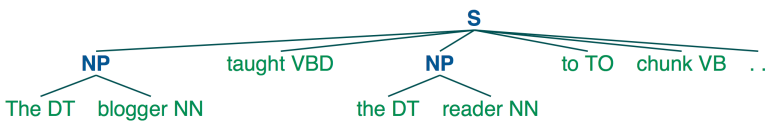
\includegraphics[width=\textwidth]{nickcdryanblog1.png}
    \caption{A sentence with simple NPs grouped}
\end{figure}\\
Let's try creating VPs now, the most simple grammar in this example would look like this:
\begin{verbatim}
    NP: {<DT>?<JJ>*<NN>} 
    VP: {<VBD>?<TO>?<VB>?}
\end{verbatim}
Run it through the algorithm above, and would you look at this:\\
\begin{figure}[htb!]
    \centering
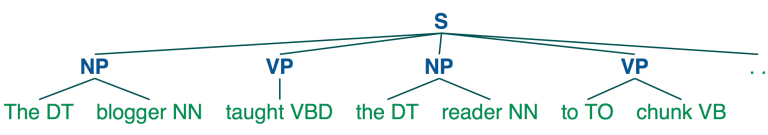
\includegraphics[width=\textwidth]{nickcdryanblog3.png}
    \caption{A sentence with simple NPs and VPs grouped}
\end{figure}\\
The issue with this grammar is that it works only with this one, simple approach proposed by the author of the blog. There are dozens of examples of custom NPs and VPs\cite{Constructing CFG} and it often turns out that the approaches are multiple-iterative and require a lot of computational complexity: \\ \\
\begin{figure}[H]
    \centering
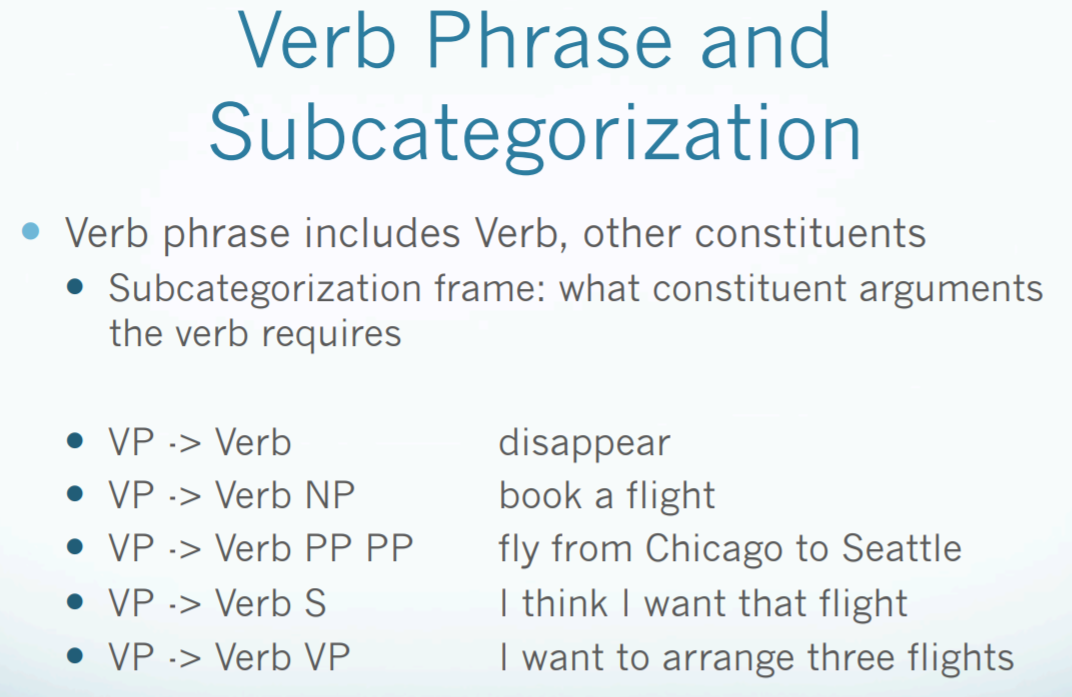
\includegraphics[width=\textwidth]{ProblemswithVPs.png}
    \caption{Some approaches at creating VP blocks}
\end{figure}
\noindent NLTK as a library supports multiple-attempt iterative approaches to grammars through the parameter "loop", where it is possible to create VPs out of VPs that did not exist on the first iteration.

\begin{verbatim}
    cp = nltk.RegexpParser(grammar, loop=2)
\end{verbatim}
Only on the second iteration the rule "VP $\rightarrow$ Verb VP" will be able to come into action, because on the first iteration no chunks were labeled as VPs to begin with. \\ \\
A few additional main blocks can be derived using this approach, such as: Adjective Phrase (ADJP), Adverbial Phrase (ADVP) and Prepostional Phrase (PP)\cite{CFG for PP etc.}. All three of those can serve as potential checkpoints on the way to finding main NPs and VPs as seen in the figure below and they have their own creation rules just as well. \\ \\
\begin{figure}[h]
    \centering
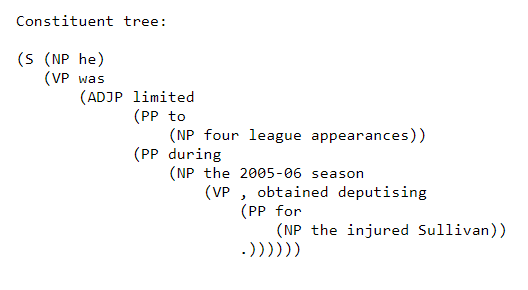
\includegraphics[width=0.6\textwidth]{NPsvsVPs.png}
    \caption{The main NP in this sentence that corresponds to the main VP is a "he". Because it is a PRP, one of the NP can be carried from the previous sentence.}
\end{figure}
\begin{figure}[H]
    \centering
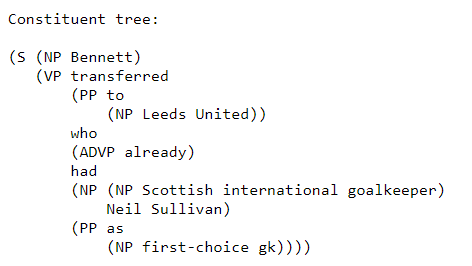
\includegraphics[width=0.6\textwidth]{NPsvsVPs2.png}
    \caption{The main NP in this sentence is "Benett", the actual agent of the sentence. Because "he" in the next sentence is a PRP, the NNP chunk of "Benett" can be carried over as the "he" of the next sentence.}
\end{figure}
\noindent Pronouns are always going to be located inside their own Noun Phrases and by looking over the influence of Verb Phrases on Noun Phrases, it is possible to prioritize certain Noun Phrases over the other when it comes to Pronouns. This approach is not always going to give perfect results, due to the fact that it's impossble to create a context-free grammar that would cover every sentence in the English Language. \\ \\
Consider the sentence "Long time no see", which has been adopted into English language, even though it is not entirely grammatically correct. It is still being used by people, even though the grammar tree of this sentence looks ambiguous.
\begin{verbatim}
    (S (VP (ADVP Long)
       time no see)
   .)
\end{verbatim}
\newpage

\subsection{Stanford Parser}
Because of edge cases, the task of creating a custom grammar can be troublesome, that's where Stanford Parser comes in. Stanford Parser can be used with NLTK library to ensure that the results will be the same as on the Stanford Parser website.\cite{Stanford Parser demo} Make note that with 3.3 version of the Stanford Parser a huge chunk of the functionality was deprecated and some hints online might be outdated. \\ \\
Stanford Parser can be used to draw neat sentence trees and extract other significant features from a sentence. \\ \\
Note that this paragraph only provides code for NLTK of versions 3.3 and above\cite{New NLTK Tokenizer}. Printing a sentence tree for a tokenized sentence can be acquired using this chunk of code:
\begin{verbatim}
    list(parser.parse(tokenized.sentence))
\end{verbatim}
Which creates the output in a format like:
\begin{verbatim}
    [Tree('ROOT', [Tree('SBARQ', [Tree('WHNP', 
    [Tree('WP', ['What'])]), Tree('SQ', [Tree('VBZ', ['is']), 
    Tree('NP', [Tree('NP', [Tree('DT', ['the']), Tree('NN', 
    ['airspeed'])]), Tree('PP', [Tree('IN', ['of']), Tree('NP',
    [Tree('DT', ['an']), Tree('JJ', ['unladen'])])]), Tree('S',
    [Tree('VP', [Tree('VB', ['swallow'])])])])]), Tree('.', 
    ['?'])])])]
\end{verbatim}
Note that this output format benefits from the extended shallow parsing labels mentioned here\cite{More labels for Stanford Parser}. \\ \\
The main labels of interest in this approach to the exercise remain NP and VP labels regardless. This process, though resource-heavy, does two things at once: returns what belongs to a given NP/VP and gives information on parts of speech that each of the words is composed of.

\subsection{Stanford Parser meets the Kaggle Task}
The sentence tree generated by Stanford Parser has multiple depth levels. One way of tackling the Kaggle assignment would be to create a specific sample space:
\begin{itemize}
    \item Find the Noun Phrase block containing at least one NNP statement that is not below the Verb Phrase and is close by to the VP phrase (as in, interrupted by only one-two blocks on the same level of the tree or one level above the VP phrase)
    \item Treat the whole chunk (including PPs inside that NP that has NNP) as the main agent of the sentence
    \item For every pronoun until the next instance of a NNP-VP block close by to one another, treat the NNP inside Noun Phrase as the person the pronoun is related to.
\end{itemize}
This cannot be the only sample space however, another sample space containing all blocks composed of NNPs should be created as well. More on this in the section \ref{Feature Space}.\\ \\
Example of this approach can be shown here (sentence 1629 from the dataset):
\begin{quote}
    In 2007, Salonga released her first studio album in seven years called Inspired, which has been certified platinum, and finished another stint in the musical Les Mis*rables on Broadway, this time as Fantine. She was scheduled to appear in a number of musical events scheduled in different countries until 2008. Salonga received the Order of Lakandula Award from Philippine president Gloria Macapagal-Arroyo in recognition of her excellence in her craft and for using \textbf{her} talents to benefit Philippine society
\end{quote}
This sentence is fairly simple to process using this approach, the highest NP and VP are on the same level in the tree, hence Salonga is the main agent of the sentence and the pronoun obviously refers to her.
\begin{figure}[H]
    \centering
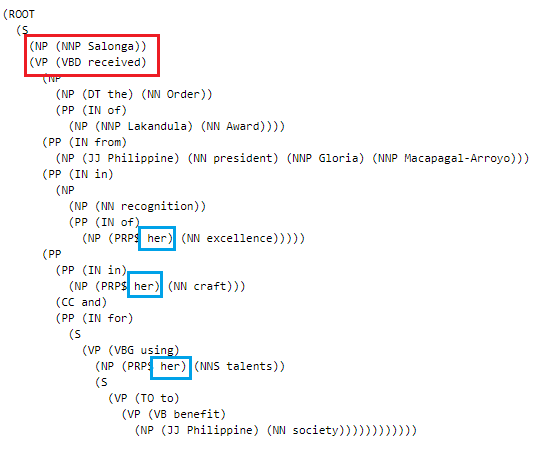
\includegraphics[width=\textwidth]{Example1.png}
    \caption{The sentence tree of this sentence, analyzed.}
\end{figure}
\noindent A more complex example would be the sentence 1630 from the dataset:
\begin{quote}
    In 1955 she added two roles to her Met repertoire: Marguerite in Charles Gounod's Faust with Thomas Hayward in the title role and Zdenka in Arabella with Eleanor Steber in the title role. After a two year absence from the Met, Fenn returned in April 1959 to portray Rosalinde in Die Fledermaus with Theodor Uppman as Eisenstein and Laurel Hurley as Adele. That role along with Mussetta became her bread and butter at the house.
\end{quote}
The algorithm described above covers it as well:

\begin{figure}[H]
    \centering
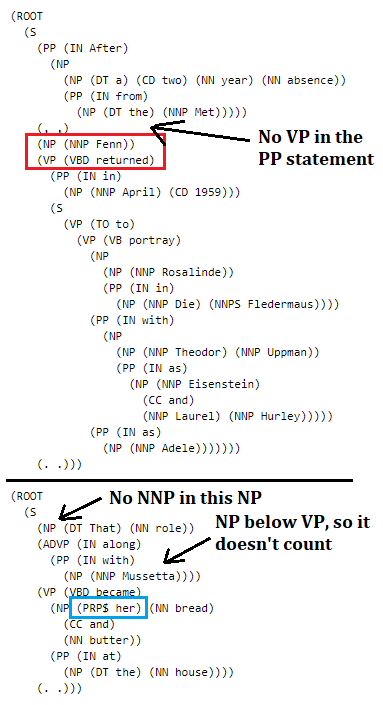
\includegraphics[width=0.6\textwidth]{Example2.png}
    \caption{The sentence tree of this sentence, analyzed.}
\end{figure}

\subsection{Challenges with this approach and how to fix them}
\subsubsection{Illegal characters}
Sentence 1610 from the dataset can present a potential challenge to an algorithm above:
\begin{quote}
    At Wimbledon, she cruised into the fourth round but was upset by Coco Vandeweghe in straight set. She then lost to Petra Kvitov* in the final at New Haven. After suffering a first round loss at the US Open to Lesia Tsurenko, it was revealed that *af**ov* was suffering from an abdominal muscle tear and a bacterial infection. She missed the Asian swing as a result and in her first match back in Linz, she lost to Andreea Mitu in straight sets.	
\end{quote}
The answer in this question is "*af**ov*" and the algorithm specified above would be able to provide a proper answer... if not for the fact that "*af**ov*" is not being treated as a NNS statement. Even more, the word is split into multiple segments that make it hard to stitch things together. Stanford Parser returns it like this: \\ \\
\begin{figure}[H]
    \centering
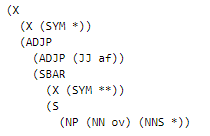
\includegraphics[width=0.5\textwidth]{Example3.png}
    \caption{The issue with supplied stars}
\end{figure}
\noindent Instead of an NNS block. A fast solution to this problem would be to replace every star in every sentence in preprocessing with a random capital letter, for example an "A". Keep in mind that in this case "*af**ov*" is one of answers, so you would need to substitute stars in that answers with capital As too. After that, the sentence will get properly analyzed and the answer will become proper.
\newpage
\begin{figure}[H]
    \centering
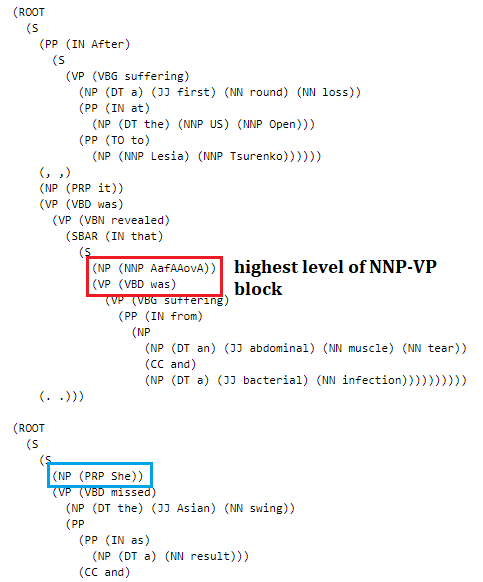
\includegraphics[width=0.65\textwidth]{Example4.png}
    \caption{Properly parsed tree}
\end{figure}

\subsubsection{Multiple NNP-VP blocks in a sentence}
Sentence 1612 presents another case worth noting in the algorithm:
\begin{quote}
    Plessy then appealed the case to the Louisiana Supreme Court, which affirmed the decision that the Louisiana law was constitutional. Plessy petitioned for a writ of error from the Supreme Court of the United States where Judge John Howard Ferguson was named in the case brought before the United States Supreme Court because he had been named in the petition to the Louisiana Supreme Court.
\end{quote}
There are two blocks of NNP-VP in the same sentence, while the pronoun "he" refers to the second one. In this case, the NNP-VP block needs to update the current NNP to the newest one for the pronoun to be correct. Make note that due to the implementation of the algorithm, Supreme Court might emerge as the NNP label for the Verb Phrase too, that's why we need to bound it so that NNP-VP relations can only be found inside the same node, not only at the same depth of the tree. \\ \\
Take note that the NNP block that the tree creates for the Judge's position is "Judge John Howard Ferguson" and the answer is "John Howard Fergusson", so it is not actually equal to what the answer supplies, too. If the phrase in the quote marks would be "Judge known as John Howard Fergusson", the whole phrase with 6 words would need to be added to the sample space, because it's all part of a NP that is directly connected to a VP.

\begin{figure}[H]
    \centering
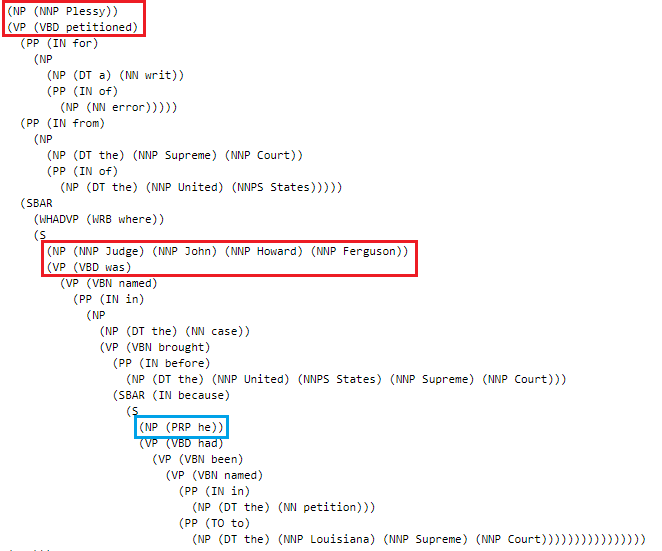
\includegraphics[width=0.65\textwidth]{Example5.png}
    \caption{Turbo problems}
\end{figure}

\subsubsection{Personal pronouns vs Possessive pronouns}
Sentence 1859 brings a difficult approach to the table:
\begin{quote}
    One More Drifter in the Snow is the sixth album and first Christmas album by Aimee Mann, released by SuperEgo Records in the United States on October 31, 2006 (see 2006 in music). It was produced by Paul Bryan and comprises covers of ``standard great Christmas classics'' and two original compositions: ``Christmastime'', written by Mann's husband Michael Penn, and ``Calling on Mary''. Grant-Lee Phillips sings with her on the track ``You're a Mean One, Mr. Grinch''.
\end{quote}
Aimee Mann, through a loophole in the algorithm is properly detected as a member of a NNP-VP block, even though the action of being "released" is not being conducted by Aimee Mann. The biggest problem with this sentence is located slightly after that point: \\ \\
\begin{figure}[H]
    \centering
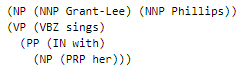
\includegraphics[]{Example6.png}
    \caption{Mega turbo problems}
\end{figure}
\noindent A newly created NNP-VP block is being initialized just before the pronoun, leading the pronoun to be connected to a wrong NNP-VP block. Luckily, the Stanford Parser allows to distinguish between PRP and PRP\$ objects, where PRP objects (personal pronouns) do not refer to NNP-VP blocks created just before it, while PRP\$ objects (possessive pronouns) can refer to them.\\ \\
As an example, consider two sentences. \\ \\
\begin{figure}[H]
    \centering
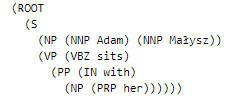
\includegraphics[]{Example7.png}
    \caption{Personal pronoun}
\end{figure}
\begin{figure}[H]
    \centering
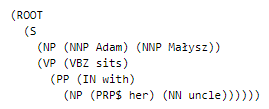
\includegraphics[]{Example8.png}
    \caption{Possessive pronoun}
\end{figure}

\noindent In the first example, Adam Małysz is not the agent to whom the pronoun "her" belongs, while in the second one Adam Małysz is the actual "her" of the sentence. Because of that, a new rule has to be erected:
\begin{quote}
    Personal pronouns (PRP) need to have a delay of at least one word from the verb when considering that they can be the agents of sentences. Possessive pronouns (PRP\$) on the other hand do not need it.
\end{quote}
\subsubsection{Having to pick neither}
This case follows directly from the previous example, consider sentence 1627:
\begin{quote}
    The rank was: #1 Megumi Ohori, #2 Yukari Sato, #3 Kayo Noro, #4 KONAN, #5 Kazumi Urano, #6 Haruka Umeda, #7 Serina, #8 Mami Kato, #9 Haruka Kohara, #10 Ito Kana, #11 Akita Kazue, #12 Fukuyama Sakura. However, Fukuyama Sakura left the group and Chen Qu replaced her on the performance.
\end{quote}
The actual agent in the sentence containing "her" is Fukuyama Sakura, but it's not any of the answers supplied in the dataset. Because neither Fukuyama Sakura and Chen Qu are answers to this question, it's easy to mark the answer as "neither". Keep in mind that in this case the approach that involves not considering Chen Qu because "her" is a PRP and shows up as the first word after the Verb Phrase.\\ \\
Sadly though, in this case an amount of NNPs that would get added to sample space of regular NNPs is huge and might influence the solution's probability rates not in our favor. This example is worth considering when trying to empirically adjust probabilistic values for an option being selected more than the other options. \\ \\
Sentence 1871 presents another interesting case:
\begin{quote}
    As well he reported that she ``admitted to Bersih receiving some money from two US organisations -- the National Democratic Institute (NDI) and Open Society Institute (OSI) -- for other projects, which she stressed were unrelated to the July 9 march.'' It is believed that former US ambassador to Malaysia had lobbied strongly the Neo Cons including Al Gore, Paul Wolfowitz and Madeline Albright to award Sreenevasan the 'Woman of Courage' award from Hillary Clinton and First Lady Michelle Obama. \textbf{She} is a member of the Malaysian Intellectual Property Association, the International Association for the Protection of Intellectual Property (AIPPI), as well as the Asian Patent Attorneys Association (APPA).
\end{quote}
Bolded "she" related to US ambassador to Malaysia, but the two answers provided are "Hillary Clinton" and "Michelle Obama". Luckily, the algorithm does not consider either Hillary Clinton or Michelle Obama to be agents of the sentence, so both of those can be crossed out. Keep in mind that according to this algorithm, "former USA ambassador to Malaysia" should form its own NNP-VP block, even though "to Malaysia" would be a PP block in itself. The reason for this is that this PP is located inside an NP block that is next to a VP block.

\subsubsection{Me and a couple of other people out of which one is one of the possible answers to mark in this painfully long entry into the sample space that machine learning will learn from}
Consider sentence 59:
\begin{quote}
    Alleway played 857 minutes in 11 matches including 9 starts. The defence conceded a total of only 5 goals in the regular season and the finals. In March 2016, Alleway and Melbourne City teammate Steph Catley joined the NWSL's newest expansion club the Orlando Pride. Orlando Pride coach Tom Sermanni gave Alleway her first cap for Australia when he was coach of the Matildas in 2010.
\end{quote} \\ \\
\begin{figure}[h!]
    \centering
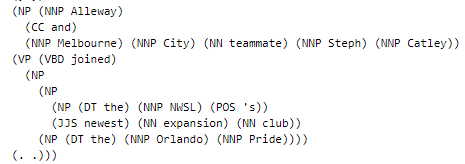
\includegraphics[]{Example9.png}
    \caption{That NP seems pretty long...}
\end{figure}
In this example both Alleway and Steph Catley are possible answers. The phrase "Alleway and Melbourne City teammate Steph Catley" is uploaded to the sample space. There are two ways to make the example print a proper answer:
\begin{itemize}
    \item Prioritize the first NNP words when using Machine Learning layer to deliver adequate answers
    \item Stop considering the next words in NP blocks after a CC object has been found
\end{itemize}
Both can be used to solve the issue. A similar problem occurs in sentence 1998
\begin{quote}
    The plot of the film focuses on the life of a Chinese American family who struggles with identity. The mother, Doris Chu, has undergone blepharoplasty, or ``double eyelid'' surgery, and the oldest of two daughters, Mei, has trouble understanding her mother's actions.
\end{quote}
Where the block uploaded to the sample space will consist of "the oldest of two daughters, Mei", where Mei is one of the possible answers. The only NNP element in that sample space is "Mei", so Mei gets selected as an answer to "her" pronoun.

\subsubsection{Paragraphs that begin with a pronoun}
Sentence 268 has an interesting approach to the problem:
\begin{quote}
    In \textbf{her} mainly positive review of Haythornthwaite's paper 'Learning, Culture and Community in Online Education: Research and Practice', Nora Wright of the University of California found one problem with the paper, in that it appears less approachable to students and researchers than the content would suggest.
\end{quote}
Even though there are no NNPs before "her", it quite clearly refers to Nora Wright of the University of California, which should get added to the sample space regardless. A new rule needs to be added to the program, stating that
\begin{quote}
    If no NNP has been found before a pronoun, the first NNP corresponds to the pronoun mentioned before.
\end{quote}

\subsubsection{The depth of the tree vs the agent}
The depth of the tree needs to be one of the parameters inside Machine Learning sample space. Consider sentence 293:
\begin{quote}
    A woman comes to Mel's shop to sell antiques from a house she's moving from after the death of her daughter (from an illness). Melinda very quickly discovers that the house is haunted by violent spirits after Ned gets hurt there-which doesn't go down well with Delia- and she realizes that the ghost of the little girl (Cassidy) is being trapped there.	
\end{quote}
Even though Melinda begins as the main agent of the sentence, she is replaced by Ned, who is several layers into the sentence tree below. This is the reason why the depth inside the tree of each NNP is a vital factor for calculating a probabilistic outcome of a given problem.
\begin{figure}[H]
    \centering
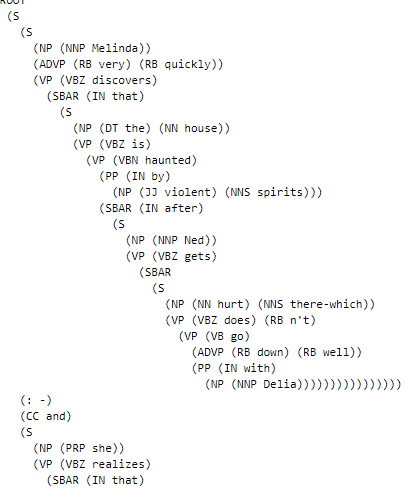
\includegraphics[width=0.65\textwidth]{Example10.png}
    \caption{The difference in depths is huge...}
\end{figure}

\noindent Melinda and "she realizes" are one depth level apart, while Ned is several levels down the tree. This is the only reason why we can attempt to attribute the "she" in this case to Melinda. A new rule can be set into place:
\begin{quote}
    If a pronoun is several layers below the pronoun in the same sentence of a tree, it does not influence the pronoun's preference.
\end{quote}

\section{Machine Learning Challenges}
Because the chunks of text that are provided to us are multi-sentence, the most important challenge of this approach is to connect each pronoun (PRP) into the most significant named chunk (NNP) from the previous or the next sentence. \\ \\
Some sentences span for such a long time, that even tokenization into separate sentences will not do enough of the job and the sentences might need to be divided by "," signs just as well as "." signs. This creates its own set of problems, because, as shown in this very sentence, some comma-split sentences might span over a single word and by setting the agent tracking to just one sentence before a given sentence, the agent will be lost. \\ \\
Even though the sections above cover a huge chunk of English grammar rules, paragraphs like 1948 containing passive voice will not return reliable results at all. For this, a different method has to be utilized. \\ \\
Managing edge cases (star signs, typos) when a Context-Free grammar will not be able to return a clear answer on who is an agent in this sentence will require a more probabilistic approach. Distances between delimiters, NPs and VPs, pronouns and NNPs might be used to determine who the main agent is. \\ \\
More complex algorithms might require a lot of computational power, making the task assignment take too long to be feasible. 
\section{Feature Space contents} \label{Feature Space}
To my mind, the algorithm will need the following chunks of data to be sent to the Feature Space:
\begin{itemize}
    \item All NNPs in sentence and their locations within the sentence
    \item A separate category for NNPs that are in a NP node that is close by to a VP node, in order (2.5.2 example: Plessy, Judge John Howard Fergusson)
    \item The heights of each of the discovered NNP-containing NP blocks in a tree
    \item The pronoun in question, its location and the depth into the tree
\end{itemize}
Features belonging to the second category should have an increased priority over the ones in the first group, but if no features from the second group are found at all, features from the first category might be considered. A result of this algorithm needs to be a probability at all times considering at least those two factors:
\begin{itemize}
    \item The NNPs from the second category contesting the depths into the tree of pronouns (as per 2.5.7)
    \item The amount of NNP blocks that are unmarked to the second category vs how probable it is that a pronoun from the second category will be valid
\end{itemize}
There is no method to calculate respective coefficients with a method other than an empirical approach, so an algorithm to calculate this needs to be created and then adequately adjusted based on results of the algorithm vs perfect results.

 
\begin{thebibliography}{9}
\bibitem{Tokenization}
\href{https://www.guru99.com/tokenize-words-sentences-nltk.html}{Tokenization in NLTP}

\bibitem{Demo of TweetTokenizer}
\href{https://stackoverflow.com/questions/37605710/tokenize-a-paragraph-into-sentence-and-then-into-words-in-nltk}{Code and demo on Stackoverflow}

\bibitem{New NLTK Tokenizer}
\href{https://github.com/nltk/nltk/wiki/Stanford-CoreNLP-API-in-NLTK}{New NLTK Tokenizer}

\bibitem{POS}
\href{https://nickcdryan.com/2017/02/13/shallow-parsing-for-entity-recognition-with-nltk-and-machine-learning/}{More on PoS labels and chunking}

\bibitem{POS labels}
\href{https://medium.com/@gianpaul.r/tokenization-and-parts-of-speech-pos-tagging-in-pythons-nltk-library-2d30f70af13b}{List of all the PoS labels}

\bibitem{Constructing CFG}
\href{http://courses.washington.edu/ling571/ling571_WIN2015/slides/ling571_class2_grammar.pdf}{More on constructing Context-Free Grammars}

\bibitem{CFG for PP etc.}
\href{https://people.cs.umass.edu/~brenocon/inlp2017/lectures/16-cfg-exercise.pdf}{Context-free Grammars for VP, NP, PP, ADJP, ADVP and others.}

\bibitem{Stanford Parser demo}
\href{http://nlp.stanford.edu:8080/parser/index.jsp}{Demo of Stanford Parser working}

\bibitem{More labels for Stanford Parser}
\href{https://gist.github.com/nlothian/9240750}{More labels in Stanford Parser}
\end{thebibliography}
\end{document}
